\section{Quasi-classical approximation}
	\subsection{Problems}
		\subsubsection{Exponential potential}
			\begin{figure}[!h]
				\centering
				\begin{tikzpicture}[scale=1,cap=round,>=latex]
\draw [<->] (0, 3) -- (0, 0) -- (7, 0);
\node [left] at (0, 3) {$U$};
\node [below] at (7, 0) {$x$};

\draw [line width=1.5] (0, 0) -- (2, 0) -- (2, 3/2);
\draw[domain=2:7,smooth,line width=1.5, variable=\x] plot ({\x},{3/\x});

\node [below] at (2, 0) {$a$};

\end{tikzpicture}
				\caption{Exponentially decaying potential barrier}
			\end{figure}
			For a potential barrier:
			\begin{align}
				U(x) = \left\{ \begin{aligned}
					0,\quad x < a \\
					\frac{\alpha}{x},\quad x > a
				\end{aligned}
				\right. \\
			\end{align}
			and a particle with $E > 0$, what are the reflection and transmission coefficients?
			
		\subsection{Hemisphere potential}
			\begin{figure}[!h]
				\centering
				\begin{tikzpicture}cap=round,>=latex]
	\begin{axis}[grid=none,
	axis x line=middle,
	axis y line=left,	
	enlargelimits,
	xtick={-1,0,1},
	xticklabels={$-a$, $0$, $a$},
	ytick={1},
	yticklabels={$U_0$},
	domain=-1.2:1.2
	]
	
	\addplot[no markers, line width=1.5, samples=50, domain=-1:1] {cos(deg(pi*x/2))};
	\end{axis}								
\end{tikzpicture}
				\caption{Hemisphere potential barrier}
			\end{figure}
			For a potential barrier:
			\begin{align}
				U(x) = U_0 \cos(\frac{\pi}{2a}x), \quad -a \leq x \leq a
			\end{align}
			and a particle with $E > 0$, what are the reflection and transmission coefficients?
		\subsection{Minimal transistor size}
			\begin{figure}[!h]
				\centering
				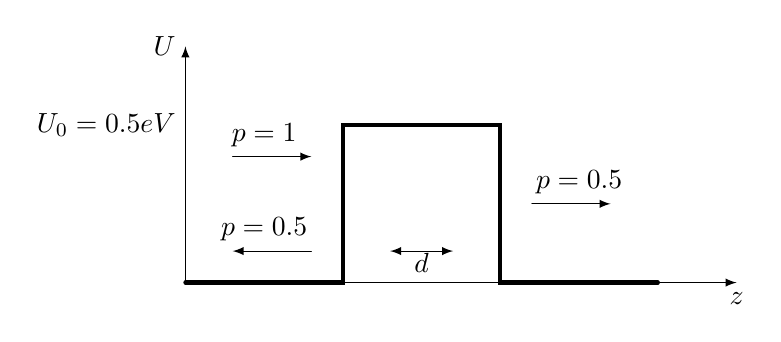
\begin{tikzpicture}[scale=2,cap=round,>=latex]
	\draw [<->] (-2, 1.5) -- (-2, 0) -- (1.5, 0);
	\node [left] at (-2, 1.5) {$U$};
	\node [below] at (1.5, 0) {$z$};
	
	\draw [line width=1.5] (-2, 0) -- (-1, 0) -- (-1, 1) -- (0, 1) -- (0, 0) -- (1, 0);
	
	\node [above] at (-0.5, 0) {$d$};
	\draw [<->] (-0.7, 0.2) -- (-0.3, 0.2);	
	
	\node [left] at (-2, 1) {$U_0 = 0.5\si{eV}$};

	\draw [->] (-1.7, 0.8) -- (-1.2, 0.8);
	\node [above] at (-1.5, 0.8) {$p = 1$};
		
	\draw [<-] (-1.7, 0.2) -- (-1.2, 0.2);
	\node [above] at (-1.5, 0.2) {$p = 0.5$};

	\draw [->] (0.2, 0.5) -- (0.7, 0.5);	
	\node [above] at (0.5, 0.5) {$p = 0.5$};
												
\end{tikzpicture}
				\caption{Model transistor}
			\end{figure}
			
			\begin{align}
				m_{el} \approx& 0.3 m_0 \\
				m_0 \approx& 10^{-30}\si{kg} \\
				p =& |\Psi|^2
			\end{align}			
			
			Calculate the size of a quantum barrier at which an electron's probability of tunneling through is equal to $0.5$ using the quasi-classical approach, and compare it to the exact solution.
		
		\subsection{Classical limit*}	
			For a potential $U(x)$ that possesses a certain number of bound states with energies $E_n$, in the limit $n\rightarrow\infty$, we transition into classical mechanics. 
			
			How does $\Delta E = E_{n+1}-E_n$ change for $n\rightarrow\infty$?
